\documentclass[11pt]{article}
\usepackage[T1]{fontenc}
\usepackage[margin=1in]{geometry}
\usepackage{newtxtext,newtxmath}
\usepackage{microtype}
\usepackage{graphicx}
\usepackage{booktabs}
\usepackage{array}
\usepackage[font=small,skip=8pt]{caption}
\usepackage{titlesec}
\usepackage{enumitem}
\usepackage[hidelinks]{hyperref}

\setlist[itemize]{leftmargin=1.25em,itemsep=0.35em,topsep=0.45em}
\setlist[itemize]{before=\raggedright}
\captionsetup[table]{position=above}
\titleformat{\section}{\large\scshape\raggedright}{\thesection.}{0.7em}{}
\titleformat{\subsection}{\normalsize\scshape\raggedright}{\thesubsection}{0.6em}{}
\titlespacing*{\section}{0pt}{1.5em}{0.6em}
\titlespacing*{\subsection}{0pt}{1.1em}{0.35em}
\setlength{\parindent}{0pt}
\setlength{\parskip}{0.55em}
\setlength{\emergencystretch}{2em}
\urlstyle{same}
\newcommand{\attack}[1]{\texttt{attack-}\allowbreak\texttt{#1}}

\begin{document}

\begin{center}
{\LARGE Direct Publication for Offline Ballots\par}
\vspace{0.55em}
{\Large An Executable Research Prototype\par}
\vspace{1.15em}
{\large Jo\~ao Henrique Menezes Silva Boia\par}
\vspace{0.35em}
Independent researcher\par
\vspace{0.2em}
October 2026
\end{center}

\vspace{0.6em}
\begin{center}
{\large\scshape Abstract}
\end{center}
\begin{quote}
This paper specifies a direct-publication protocol for offline encrypted ballots using established cryptographic primitives. It distinguishes the protocol primitives from the investigated publication decision and from implementation findings: the protocol uses ballot proofs, signed batches, and threshold decryption; the design choice is to publish the machine-signed batch directly rather than hand it to an intermediary for forwarding; and the implementation provides eight attack commands alongside focused regression tests and a small historical measurement run. The receipt is issued after candidate selection and before the voter chooses CONFIRM or TEST. A TEST reveals and spoils that ballot; a confirmed ballot remains encrypted. Three of five trustees contribute shares to decrypt the aggregate, while a separate verifier checks supplied receipts and recomputes the tally from public evidence. The run contains six confirmed ballots, one spoiled ballot, and three samples per measured operation. It is not a security proof, deployment evaluation, or new cryptographic primitive, and it does not imply that existing elections lack audits.
\end{quote}

\section{Introduction}
The prototype separates encrypted ballot creation, publication, threshold decryption, and verification. This paper documents those interfaces and executable checks. Signature verification authenticates bytes under a supplied key and domain; it does not establish voter intent, guarantee delivery, or establish the independence of the party supplying the key or verifier.

The path studied here has four roles. The offline machine prepares the encrypted ballot and receipt. A public contract records the machine's signed batch. Five trustees hold shares of the decryption key, and any three can open the sum. An independent verifier recomputes the result from published evidence. The machine publishes its own batch. A poll worker may enable the simulated connection after the close, but that person does not receive the votes. The signature check depends on the signed bytes and trusted verification key, not on how the bytes were transported.

This is a specification and local integration demonstration, not a proposal to replace existing election procedures. The protocol uses established ballot and threshold-cryptography constructions; the design contribution investigated here is direct publication of a signed batch. The local contract checks registered signers and one-batch rules, and the verifier checks supplied evidence and tally consistency. These are implementation checks, not evidence that the protocol is secure in a deployed election.

The demo implements publication by the machine account; it does not evaluate institutional arrangements. The machine must be able to reach the board, and the board and its data must remain available. The 3-of-5 interface permits tally decryption with three shares, but any three colluding trustees can also decrypt individual ciphertexts. The local demonstration uses one chain process controlled by one operator.

\section{Implementation and evidence}
\subsection{Roles}
Table~\ref{tab:roles} describes the prototype's implemented interfaces, not a comparison with an electoral system. The Brazilian electoral authority documents online publication of BUs, RDV, and logs, a published QR-code format that third parties may implement, and procedures for source-code inspection~\cite{tseAudit}. This citation establishes the documented procedures; it is not an independent audit of their execution.

\begin{table}[ht]
\centering
\caption{Implemented interfaces and the evidence each one handles.}
\label{tab:roles}
\small
\begin{tabular}{@{}>{\raggedright\arraybackslash}p{0.16\textwidth}>{\raggedright\arraybackslash}p{0.40\textwidth}>{\raggedright\arraybackslash}p{0.38\textwidth}@{}}
\toprule
Step & Operation & Evidence or check \\
\midrule
Ballots & Machine encrypts the selection & Bit and exactly-one proofs \\
Receipt & Issued after selection, before CONFIRM or TEST & Signed ciphertext commitment \\
Publication & Machine submits its finalized batch & Domain-bound batch signature \\
Board & Records one batch per machine & Registry, signature, deadline \\
Opening & Trustees submit aggregate contributions & Aggregate-bound decryption proofs \\
Verification & Separate program processes public files & Batch completeness, receipts, proofs, tally \\
\bottomrule
\end{tabular}
\end{table}

If exactly the same signed bytes are forwarded by another party, the signature check at the destination is unchanged. This is a property of signature verification, not an experimental comparison or a finding about institutional independence. Publication in this implementation requires the machine-account credential, connectivity, and an accepting board. A receipt holder can check whether the committed ciphertext appears in the supplied evidence; that check alone does not establish voter intent.

The dealer is trusted, the demonstration process holds all five shares, and any three colluding trustees can decrypt individual ciphertexts; the aggregate-only interface is not a cryptographic barrier to collusion. The verifier requires complete authentic evidence. A malicious machine can encrypt a choice different from the voter's intent. Since the receipt follows selection, detecting this requires an independent voter comparison with the intended candidate; the TEST consistency check alone does not establish intent. One local chain operator can censor or reset the chain, and copied event data is not proof of independent consensus.

\subsection{Threat model and claim boundaries}
The assets are choices and randomness before disclosure, key shares, batch integrity, retained receipts, complete board evidence, and the tally. Considered adversaries may control a machine, alter or omit transport data, submit rogue or duplicate batches, announce false totals, supply malformed proofs, censor evidence, collude as trustees, coerce voters, or control the local chain and host. The prototype has no voter roll, eligibility checks, turnout reconciliation, or one-person-one-vote enforcement.

\textbf{Assumptions.} The manifest, trustee registry, public key, and exported board evidence must be authentic and complete. A trusted dealer creates 3-of-5 shares; there is no distributed key generation. Machine and host are not remotely attested. The local chain is one process, not independent consensus. TEST selection must be unpredictable to a malicious machine for challenge value, and voters must be able to compare the candidate independently. The integration examples do not establish these assumptions.

\textbf{Properties checked.} The contract checks registration, signatures, deadlines, and append rules. The off-chain verifier checks ballot proofs and openings, receipt signatures and inclusion, supplied partial proofs, and tally consistency. Signatures make edits to signed bytes detectable in both paths; they do not prevent omission or guarantee delivery. These properties do not establish eligibility, coercion resistance, or availability.

\textbf{Collusion and post-detection limits.} Any three trustees can decrypt arbitrary ciphertexts despite the aggregate-only workflow. The dealer is trusted, the demo process holds all shares, and the chain operator can censor or reset the local chain. The contract does not verify ballot or trustee proofs. Missing machine batches, invalid ballots, invalid supplied receipts, or inconsistent event hashes stop the audit without totals; the verifier does not discard ballots to produce a partial election result. Invalid trustee contributions are handled separately as described below. There is no automatic election annulment or dispute-resolution procedure. Media loss, withholding, access costs, exception handling, and preservation are operational scenarios, not findings about Brazil. The cited Brazilian rules describe integrity checks, designated technical recovery, recovery from available machine or media records or a printed BU, reasoned exception records, and preservation~\cite{tseResolution}.

\section{Protocol}
The group is RFC~3526 group~14: a 2048-bit prime $p$, order $q=(p-1)/2$, and generator $g=2$~\cite{rfc3526}. Secret exponents lie in $\mathbb{Z}_q$, and the public key is $y=g^x$. For a bit $m$ and fresh randomness $r$, exponential ElGamal is
\begin{equation}
  \operatorname{Enc}_y(m;r)=(a,b)=(g^r,\, y^r g^m) \pmod{p}.
\end{equation}
A ballot is one ciphertext per candidate. Each ciphertext carries a Fiat--Shamir OR proof that it encrypts zero or one. The challenge binds a domain separator, the election identifier, the public key, the whole ordered ciphertext vector, and the candidate index, so a proof cannot be moved to another election, key, ballot, or position. A second proof shows that the candidate bits sum to one. With $A=\prod_i a_i$, $B=\prod_i b_i$, and witness $R=\sum_i r_i \bmod q$,
\begin{equation}
  \log_g A = \log_y(B/g) = R \pmod{q}.
\end{equation}
The transcript is canonical JSON, hashed with SHA-256, and reduced modulo $q$. Subgroup membership, scalar ranges, encodings, and the proof equations are checked before a ballot is accepted. The equality proof follows Chaum and Pedersen~\cite{chaum1993wallet}. The sharing follows Shamir~\cite{shamir1979}. Neither construction is new here.

\subsection{Receipt, then confirm or test}
The machine encrypts the selected choice and signs the receipt after selection but before the voter confirms or tests. The receipt binds the election, the chain, the board, the machine account, and a SHA-256 commitment to the ordered ciphertext vector. Proof bytes are not part of that commitment. A 20-hex-character code is an 80-bit locator for lookup. It is not the binding value. Verification uses the full digest and the signature. Because the receipt follows selection, it is not independent evidence of what the voter intended.

Before emitting a receipt, the machine checks that either decision would fit the canonical batch-size limit, including the larger TEST opening. A capacity refusal emits no receipt and leaves previously accepted ballots unchanged. This does not provide crash persistence of the machine's in-memory state.

On TEST, the machine reveals the choice and randomness and marks the ballot spoiled. The verifier recomputes the ciphertexts and checks opening consistency. The revised machine-attack command exercises two distinct cases: an inconsistent opening fails cryptographically; a valid opening of a substituted choice passes cryptographic verification but fails a separate comparison with remembered voter intent. Disabling that comparison makes the second demonstration fail to detect the substitution. This is a simulated trusted comparison, not a validated human interface. Tested ballots do not count, and the voter votes again. On confirmation, randomness stays undisclosed. The receipt does not prove a physical button press or eligibility.

\subsection{Direct publication}
Local voting closes first. The voting program cannot enable transport before that close. After the close, the machine publishes one signed batch before the upload cutoff. The cutoff is not the same event as the local close: machines do not have to finish closing before any machine may upload. When the batch deadline passes, the board closes and a snapshot is fixed. Trustee shares are accepted only after that snapshot and before a separate deadline.

The batch is signed by the same secp256k1 account that submits the transaction. The EIP-191 digest binds the chain, the board, the election, and the payload. The contract checks the signer, the deadline, and the one-batch rule, then emits the payload and its hash. The verifier checks the event and the signature. Nothing in this step decrypts a ballot.

The demonstration submits the finalized batch without first writing a transport file. An optional carrier copy is staged, flushed, and file-synced before atomic no-clobber publication in the same directory. A failed write leaves no completed-looking destination and can be retried. Failure to create the optional copy is reported and does not stop direct submission of the other machine's batch. This mechanism does not guarantee directory-entry durability after power loss, recover lost memory, or make all copies available. Possessing the carrier does not supply the machine-account credential required for submission.

\subsection{Opening only the sum}
The verifier multiplies the ciphertexts of cast ballots after the board has closed. Spoiled ballots stay out. For a product $(A,B)$ and a trustee share $s_i$, trustee $i$ posts $D_i=A^{s_i}$ and a Chaum--Pedersen proof that $\log_g VK_i=\log_A D_i$, where $VK_i=g^{s_i}$. Each proof binds the election, the aggregate digest, the trustee index, the candidate, the key, the ciphertext, and the commitments. For a set $S$ of three trustee indices,
\begin{equation}
  \lambda_i=\prod_{\substack{j\in S\\ j\ne i}}\frac{-j}{i-j}\pmod{q},
  \qquad D=\prod_{i\in S} D_i^{\lambda_i}.
\end{equation}
The plaintext group element is $B/D=g^T$. The verifier solves for $T$ inside the declared tally bound. The result is the aggregate. It is not a cryptographic guarantee against three trustees who decide to decrypt some other ciphertext.

A registered trustee may submit once. The revised board pins a digest only after three distinct trustees have posted that digest; one or two early conflicting submissions do not establish the pin. This agreement is not a proof of mathematical correctness. The verifier recomputes the aggregate from all audited ballots, requires the pin to match it, and checks each contribution. Invalid trustee payloads, aggregate bindings, or proofs are excluded and their indices appear in \texttt{rejected\_trustees}. At least three distinct valid contributions are still required. Duplicate trustee events or corrupted event hashes stop the audit. A successful report with rejected trustees verifies the tally from the valid threshold, not the validity of every submitted contribution.

\section{What the checks catch}
The eight commands below are integration examples showing that corresponding checks fire in this implementation. They are not a security proof. The fail-closed ballot checks and threshold-contribution exclusions described above are program behavior, not an adjudication or automatic annulment procedure.

\begin{itemize}
\item \textbf{TEST opening and intent.} The command separately demonstrates rejection of an inconsistent opening and a valid substituted-choice opening detected only by a simulated independent intent comparison (\attack{machine}). Untested ballots and human comparison effectiveness are not covered.
\item \textbf{Edited transport.} Changing the signed bytes invalidates the signature, and the contract rejects the submission (\attack{transport}).
\item \textbf{Dropped ballot.} A retained receipt that is absent from the signed batch fails the check (\attack{drop-vote}).
\item \textbf{False tally.} An announced total that disagrees with the recomputation is rejected (\attack{tally}). The verifier uses the public evidence, not a private list of expected choices.
\item \textbf{Two selections.} A ballot with two selected candidates fails the exactly-one proof (\attack{double-vote}). The proof does not stop someone from submitting several valid ballots.
\item \textbf{Second batch.} The contract rejects another batch from a registered machine while the upload window is still open (\attack{duplicate}).
\item \textbf{Unknown machine.} The contract rejects a signer that was never registered (\attack{rogue-machine}). Registration itself is an external anchor.
\item \textbf{Early network.} The voting program cannot enable the simulated transport before the close (\attack{early-network}). This is a property of the software state, not of a physical switch.
\end{itemize}

If each ballot is tested independently with probability $p$ after the receipt exists, and $k$ ballots were altered, the chance of catching at least one alteration is $1-(1-p)^k$. Figure~\ref{fig:challenge} plots that expression. It is not a measured detection rate. It assumes the decision is unpredictable and independent of what the machine knows. It does not model coercion, correlated tests, or malware that adapts only to ballots it expects to remain untested.

\begin{figure}[t]
\centering
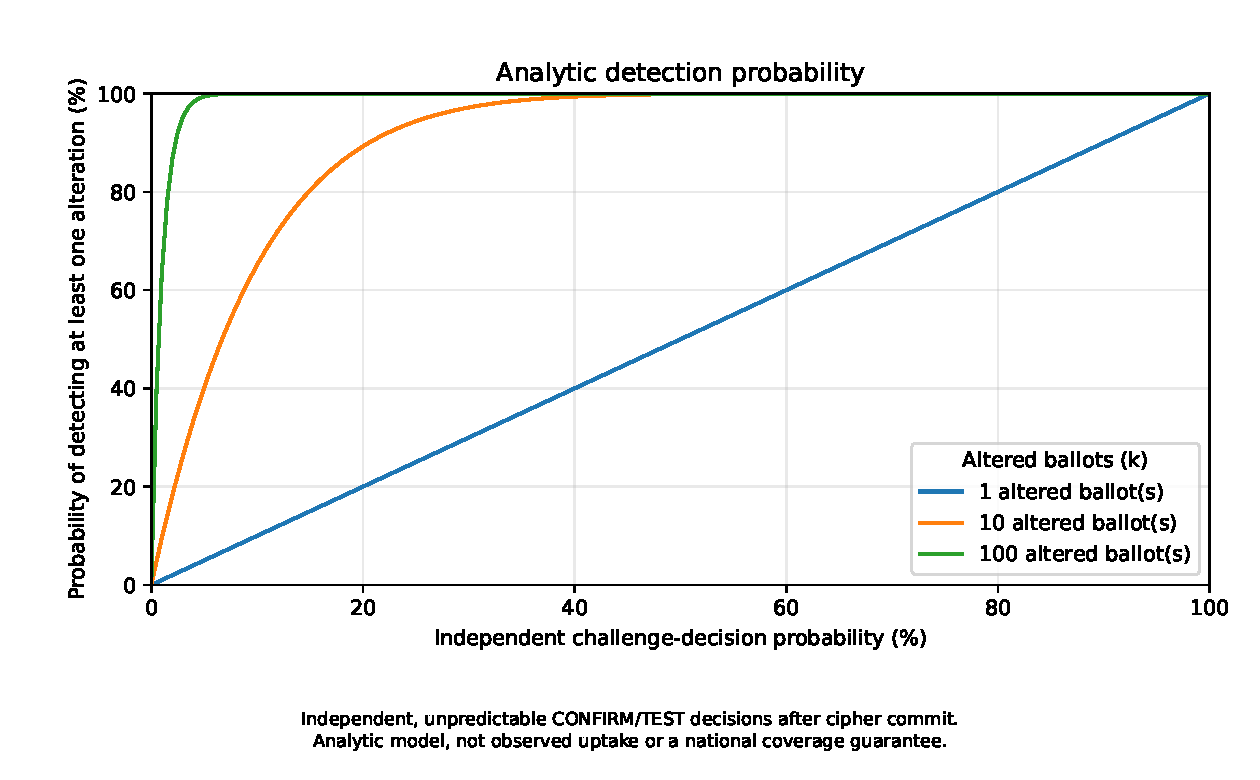
\includegraphics[width=0.78\textwidth]{figures/challenge-probability.pdf}
\caption{Analytic probability $1-(1-p)^k$ of detecting at least one altered ballot when tests are independent and chosen after the receipt exists. The curves are the equation, not observed detection rates.}
\label{fig:challenge}
\end{figure}

\subsection{Regression scenarios in the revised implementation}
Revision \texttt{8df8e3a} also contains focused regressions for four concrete failure paths. An artificially reduced payload limit makes the capacity boundary inexpensive to exercise: no new receipt is emitted when either decision would exceed it. Injected carrier-write and publication failures leave no partial destination, preserve existing files, and permit retry. A real local-contract scenario submits two wrong digests first, followed by three valid contributions; the verifier returns the expected tally and reports rejected trustees 1 and 2. A full synthetic election with both optional carrier writes disabled still publishes two batches and verifies totals $(2,2,2)$, with two explicit carrier warnings. These are bounded fault-injection observations, not measured attack probabilities, usability results, or evidence about another voting system.

\section{Measurements}
The implementation has an offline Python machine, a Solidity contract, and a separate Python verifier. The reported run uses one local Anvil process. These observations describe the recorded baseline implementation, not necessarily revised code; they are not a public-chain fee schedule or a benchmark across hardware. Tool installation and the first container build are excluded. The recorded environment is arm, Python~3.12.11, Anvil~1.8.5, and Darwin~27.2.0.

The run contains six cast ballots, one spoiled ballot, three candidates, two machines, two batches, and three partial decryptions. Each pure operation has three samples. Three fresh demonstration-process and node runs took 56.591~s, 56.175~s, and 56.165~s. Each sample is a fresh demonstration process and node; cache state was not controlled. Three isolated verifier processes took 17.820~s, 17.830~s, and 17.815~s.

\begin{table}[t]
\centering
\caption{Pure-operation time in seconds from three samples, rounded to three decimal places. Range is the minimum and maximum.}
\label{tab:timings}
\small
\begin{tabular}{@{}lrr@{}}
\toprule
Operation & Median (s) & Range (s) \\
\midrule
Three-candidate encryption & 0.152 & 0.151--0.152 \\
Bit proofs, including opening checks & 1.088 & 1.086--1.127 \\
Full ballot, including the sum proof & 1.137 & 1.135--1.210 \\
Public verification of one ballot & 0.827 & 0.824--0.833 \\
\bottomrule
\end{tabular}
\end{table}

Bit-proof time includes ciphertext setup and opening checks. Full-ballot time includes those proofs and the sum proof; it does not isolate the sum proof. Figure~\ref{fig:evaluation} shows the same three-sample medians and ranges. Three samples support a median and a range. They do not support a confidence interval or a prediction for another processor.

\begin{figure}[t]
\centering
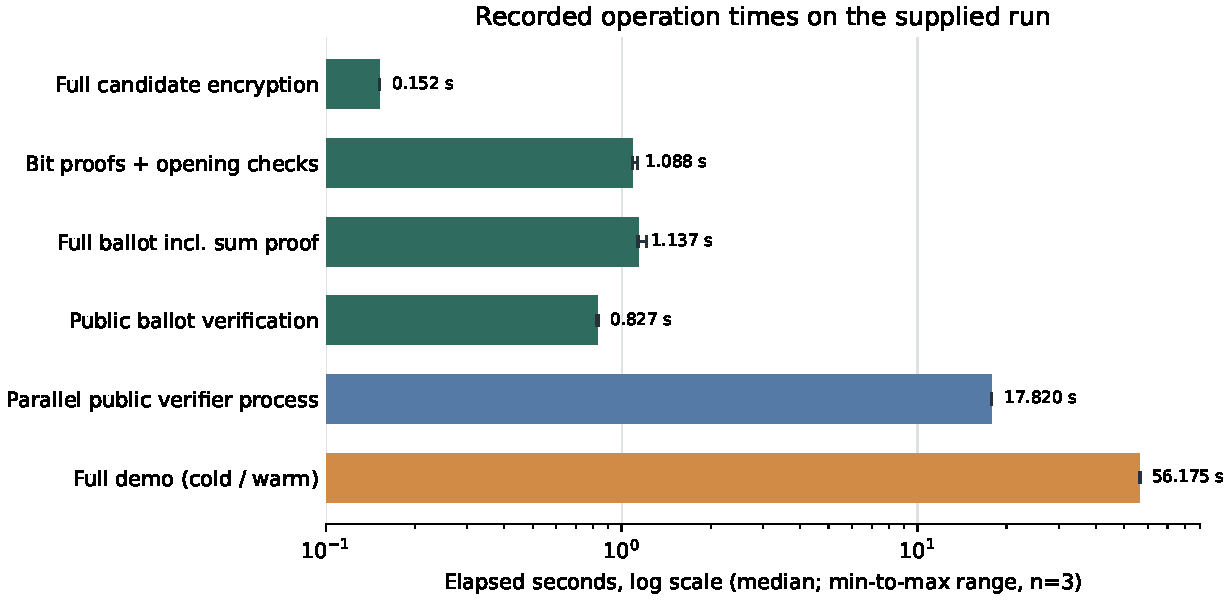
\includegraphics[width=0.88\textwidth]{figures/evaluation.pdf}
\caption{Medians and minimum-to-maximum ranges from the supplied measurement record, three samples each, rounded to three decimal places. The axis is logarithmic elapsed time.}
\label{fig:evaluation}
\end{figure}

\begin{table}[t]
\centering
\caption{Payload size and gas for the two published batches on the local chain. Gas is an execution unit, not a currency fee.}
\label{tab:gas}
\small
\begin{tabular}{@{}lrrr@{}}
\toprule
Batch & Payload (bytes) & Gas & Cast ballots \\
\midrule
First machine, mixed & 44{,}416 & 1{,}802{,}170 & 3 \\
Second machine, cast only & 32{,}217 & 1{,}314{,}280 & 3 \\
\bottomrule
\end{tabular}
\end{table}

The two payloads together contain 76{,}633 bytes, including headers and the spoiled ballot. Proof bytes in those batches total 50{,}974. One canonical cast record in the measurement file is 10{,}622 bytes. Each of the three partial decryptions used 219{,}600 gas. These are recorded baseline values, not new benchmark results for revised code.

\subsection{Scope of the measurements}
These measurements cover one small demonstration on one local Anvil process: six cast ballots, one spoiled ballot, three candidates, two machines, two batches, and three partial decryptions. The implementation's current limits are 16 machines, a tally bound of 16{,}000, and a 16~MiB payload. No large-batch, throughput, national-scale, restart-recovery, publication-outage, or accessibility experiment was performed. No linear extrapolation from these observations is warranted.

\section{Related work}
The 2008 Helios system described by Adida uses encrypted ballots and a mixnet; its remote-voting setting has a different trust boundary from a polling-place machine and does not remove coercion~\cite{adida2008helios}. Benaloh's verifiable elections are the reference for a voter checking an encrypted choice~\cite{benaloh2006simple}. ElectionGuard specifies a full system, with a different group and encryption construction; nothing here claims compatibility or equal assurance~\cite{benaloh2024electionguard}. Scantegrity~II puts end-to-end checks on optical-scan paper~\cite{chaum2008scantegrity}. vVote describes a polling-place system whose operational assumptions are not the ones implemented here~\cite{culnane2015vvote}.

Those systems address broader requirements, including credentials, paper processes, or, in the cited 2008 Helios system, a mixnet. This prototype leaves such matters out. Direct signed publication and threshold opening of the aggregate do not show that a smaller system is safer or suitable where eligibility, accessibility, and legal dispute processes are required.

Park, Specter, Narula, and Rivest argue that moving an election onto a network or a chain can add malware, coercion, censorship, and a weak dispute story rather than remove them~\cite{park2021bad}. Direct publication answers only the intermediary. It does not answer a compromised machine, a coerced voter, or a chain that refuses the transaction. Risk-limiting audits need voter-verifiable paper records~\cite{lindeman2012rla}. A ciphertext receipt does not replace those records.

\section{Limits}
The dealer is a single trusted setup. There is no distributed key generation. Three colluding trustees can read individual ballots, and the demonstration holds every share. The implementation is ordinary Python and does not protect secrets from a program that logs them. The simulated seal, power cut, reinstall, and hash comparison do not prove that a particular device ran a particular binary.

There is no voter list, eligibility check, turnout reconciliation, or one-person-one-vote check. The contract does not verify ballot proofs, trustee proofs, or tally arithmetic. Three colluding trustees can establish an incorrect pin; insufficient valid contributions stop the audit. The local chain can be reset, and an authentic complete export remains an external assumption. The revised tests cover failed optional carrier writes and conflicting trustee submissions, not arbitrary network outages, power loss, restart recovery, inaccessible verification tools, loss of every copy, or human challenge participation. A missing complete batch is rejected, not recovered. Detection provides neither automatic annulment nor a dispute remedy.

\section{Conclusion}
The implementation publishes a finalized signed batch, checks complete ballot evidence, and derives a tally from verified trustee contributions. Its executable examples document specific acceptance and rejection behavior. The historical measurements describe one small local run. These observations do not establish national readiness, institutional independence, human-verification effectiveness, or protection against a compromised machine, three colluding trustees, or a chain operator that censors publication.

\section*{Availability}
The revised executable checks are identified by source revision \texttt{8df8e3a}; the historical timing and gas record is retained from revision \texttt{f8d9358}. The recorded artifacts are \path{demo/results/measurements.json}, \path{demo/results/evidence.json}, \path{demo/results/manifest.json}, \path{demo/results/receipts.json}, and \path{demo/results/verifier-report.json}. The \texttt{Makefile} defines \texttt{make test} and \texttt{make attacks}. The revised regression sources are \path{tests/test_machine.py}, \path{tests/test_transport.py}, \path{tests/test_chain.py}, \path{tests/test_verifier.py}, and \path{tests/test_demo.py}; the intent-comparison examples are in \path{tests/test_attacks.py}. These measurements describe the baseline and are not automatically results for revised code. The code is under the Apache License~2.0. No permanent archive, DOI, arXiv posting, or remote URL is available yet; no publication is claimed.

\bibliographystyle{plain}
\bibliography{refs}

\end{document}
